\asection{Memory Results}
\label{Memory Results}
This chapter compares the efficiency of the two algorithms in terms of their memory. The amount of virtual memory used by the two algorithms are graphically 
represented, analysed and a conclusion of as to which of the two algorithm is more efficient in terms of memory is reached based on figure \ref{fig:memory_comparison}.
\begin{figure}[H]
  \begin{center}
      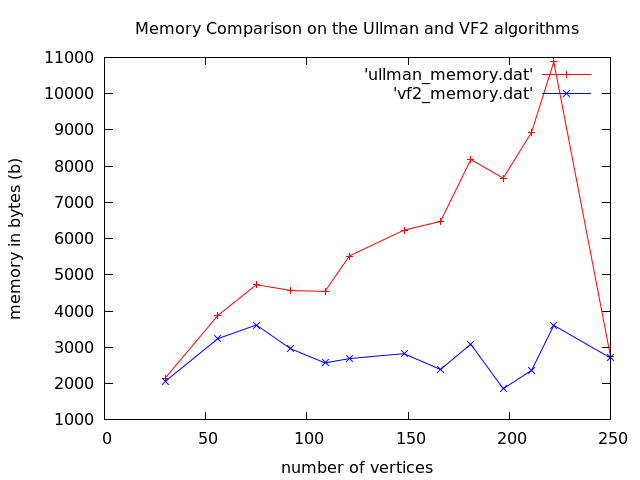
\includegraphics[width=0.8\textwidth]{memory_comparison.png}
  \end{center}    
  \caption{Graph depiting the results for the memory comparison between the algorithms}
  \label{fig:memory_comparison}
\end{figure}

\subsection{Analysis of results}
Figure \ref{fig:memory_comparison} depicts the comparison of the Ullman and the VF2 algorithms on the criteria of memory used during the execution of the graph matching processes
of the respective algorithms.\newline\newline
The virtual memory used by the the Ullman algorithm is depicted by the \textit{red} line in figure \ref{fig:memory_comparison} and the \textit{blue} line
represents the virtual memory used by the VF2 algorithm.\newline\newline
Figure \ref{fig:memory_comparison} depicts that the memory usage of the two algorithms is approximatly the same for smaller graphs of \textit{30 - 40} 
vertices. But from approximatly \textit{40} and above, it is clear that the performance of the VF2 algorithm is exceptionally superior to that of the 
Ullman algorithm. This deduction is derived from the observation on figure \ref{fig:memory_comparison}, we can see the more vertices there are in 
the graph, the more virtual memory resources is required by both graphs, but the Ullman algorithm requires a greater amount of resources than those 
used by the VF2 algorithm.\newline\newline
The superiority of the VF2 algorithm for this data set is limited, this is because when the number of vertices in the graph is approximatly \textit{220}, 
the required memory resources for both algorithms start dropping rapidly, and they finally end up requiring the same amount of memory resources.

\subsection{Conclusion}
Figure \ref{fig:memory_comparison} has provided with a graphical representation of the virtual memory required by both algorithms, and thus a way to
make deductions about the efficiency of the two algorithms in terms of memory.\newline\newline
From \ref{fig:memory_comparison}, it is clear that the VF2 is algorithm is more memory efficient than the Ullman algorithm as it requires the least amount 
of virtual memory overall for its execution.